The second test was carried out with the same configuration. Again the size of the system matrices exceeded memory and therefore there are not data points for polynomial degrees $k=2,3$ on fine grids. Table \ref{tab: l2 errors test 2} show the decreasing error norms, it shows only two degree pairs for other degree pairs behaved similarly as we can already see in figure \ref{fig: l2 errors test 2} and \ref{fig: h1 errors test 2}.
\begin{figure}[h]
\centering
	
\includegraphics[scale =0.4]{../../FEniCS/diagrams/MA2_Neilan_l2.pdf}
	\caption{$L^2$ errors for test case \ref{test sqrt} }
	\label{fig: l2 errors test 2}
\end{figure}
\begin{figure}[h]
	\centering
	
\includegraphics[scale =0.4]{../../FEniCS/diagrams/MA2_Neilan_h1.pdf}
	\caption{$H^1$ errors for test case \ref{test sqrt} }
	\label{fig: h1 errors test 2}
\end{figure}
\begin{table}[H]
	\begin{subtable}[b]{0.45\textwidth}
		\centering
		\pgfplotstabletypeset[
		columns={iterations, l2error, h1error,N},
		    every row 0 column 0/.style={set content=init},
		]{\MATwodegTwoTwo}
    	\caption{Error for $k=2, k_{DH}=2$}
   \end{subtable}
   ~
	\begin{subtable}[b]{0.45\textwidth}
		\centering
		\pgfplotstabletypeset[columns={iterations, l2error, h1error,N},
		    every row 0 column 0/.style={set content=init},
		]{\MATwodegThreeThree}
	\caption{Error for $k=3, k_{DH}=3$}
	\end{subtable}
	\caption{Errors for test case \ref{test sqrt}}
	\label{tab: l2 errors test 2}
\end{table}

\begin{table}[H]
\centering
\begin{subtable}[b]{0.45\textwidth}
	\pgfplotstabletypeset
	{
		k $k_{DH}$ {numerical order}
		2 1 1.55213
		2 2 1.63088 
		3 2 1.64644
		3 3 1.64841
	}
	\caption{numerical order in $L2$ norm}
	\end{subtable}
	\begin{subtable}[b]{0.45\textwidth}
	\pgfplotstabletypeset
	{
		k $k_{DH}$ {numerical order}
		2 1 0.465187
		2 2 0.473759
		3 2 0.475829
		3 3  0.495565
	}
	\caption{numerical order in $H1$ norm}
	\end{subtable}
	\caption{numerical order with jump penalty in test \ref{test smooth}}
\label{tab: order jump test 2}
\end{table}

Switching the penalisation of gradient jumps on the method performs again well, its results are shown in figure \ref{fig: l2 errors test 2 jump} and the tables . 
\begin{figure}[H]
\centering
\begin{subfigure}{\textwidth}
\centering
	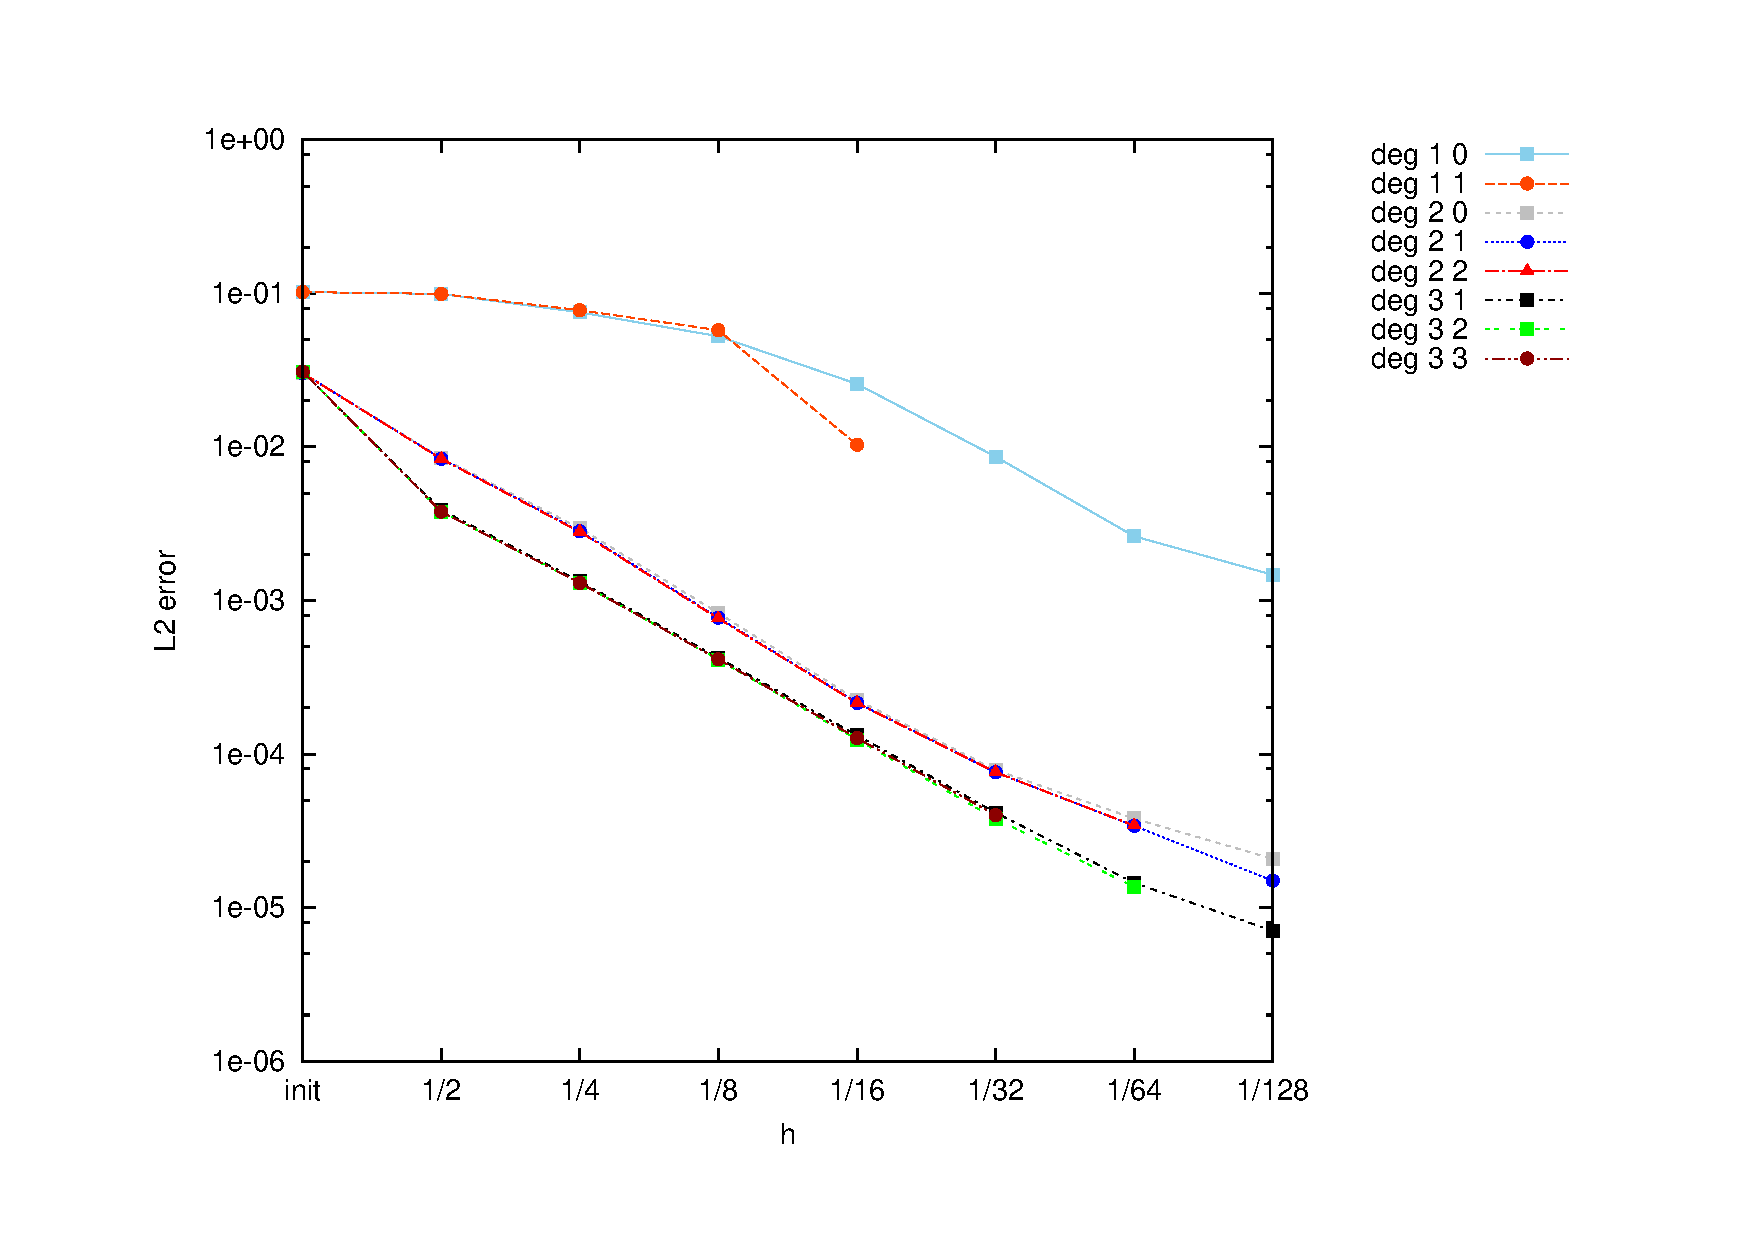
\includegraphics[scale =0.4]{../../FEniCS/diagrams/MA2_Neilan_GradJump_l2.pdf}
\end{subfigure}

\begin{subfigure}{\textwidth}
\centering
	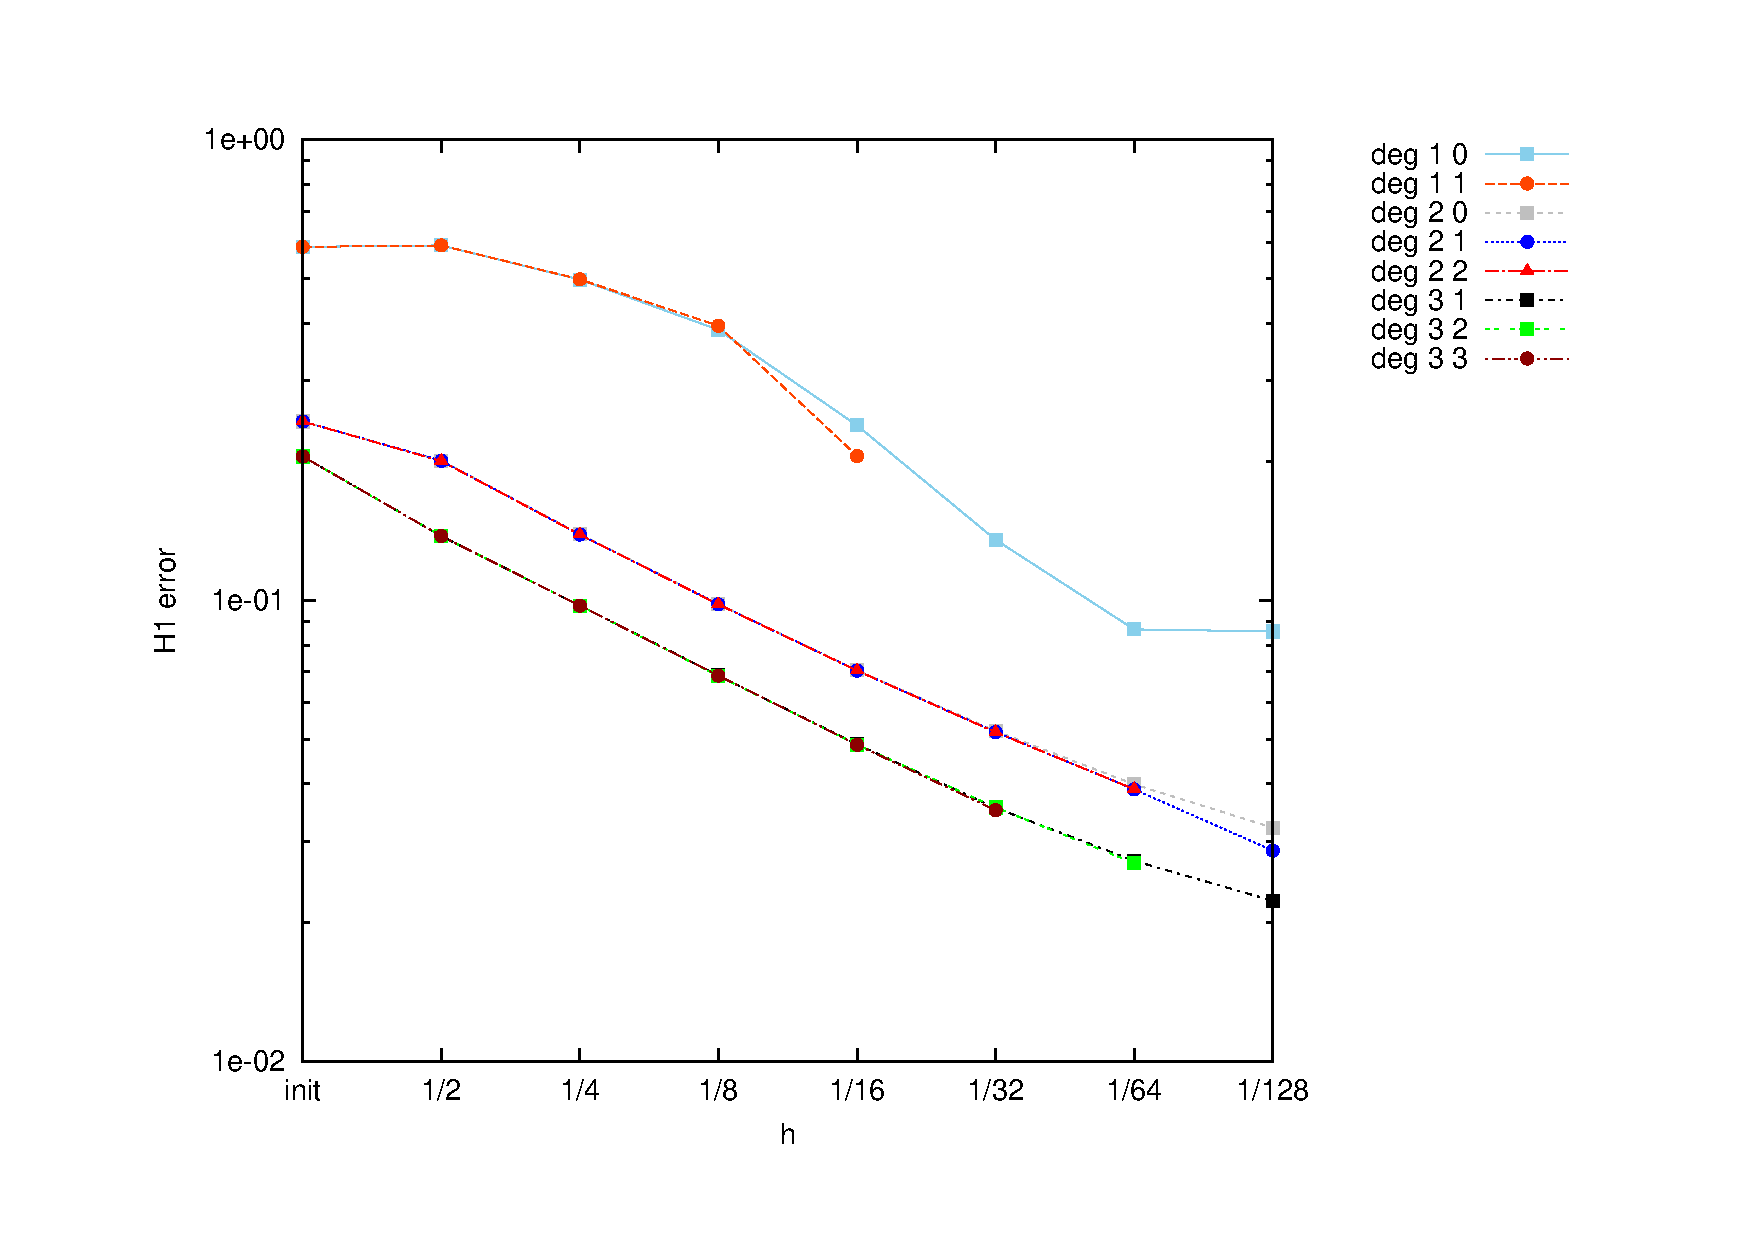
\includegraphics[scale =0.4]{../../FEniCS/diagrams/MA2_Neilan_GradJump_h1.pdf}
\end{subfigure}
	\caption{$L^2$ and $H^1$ errors for test case \ref{test sqrt} and additional gradient jump penalty}
	\label{fig: l2 errors test 2 jump}
\end{figure}
\begin{table}[H]
	\begin{subtable}[b]{0.45\textwidth}
		\centering
		\pgfplotstabletypeset[
		columns={iterations, l2error, h1error,N},
		every row 0 column 0/.style={set content=init},
		]{\MATwoJumpdegTwoTwo}
		\caption{Error for $k=2, k_{DH}=2$}
	\end{subtable}
	~
	\begin{subtable}[b]{0.45\textwidth}
		\centering
		\pgfplotstabletypeset[columns={iterations, l2error, h1error,N},
		every row 0 column 0/.style={set content=init},
		]{\MATwoJumpdegThreeThree}
		\caption{Error for $k=3, k_{DH}=3$}
	\end{subtable}
	\caption{Errors for test case \ref{test sqrt} with additional }
	\label{tab: l2 errors test 2 jump}
\end{table}

As we can see the results do not alter between the method with or without additional penalty on the gradient. Therefore also the numerical orders are almost identical.  
%\begin{table}[H]
%\centering
%\begin{subtable}[b]{0.45\textwidth}
%	\pgfplotstabletypeset
%	{
%		k $k_{DH}$ {numerical order}
%		1 0 1.03719 
%		2 1 1.55213
%		2 2 
%		3 2 
%		3 3 
%	}
%	\caption{numerical order in $L2$ norm}
%	\end{subtable}
%	\begin{subtable}[b]{0.45\textwidth}
%	\pgfplotstabletypeset
%	{
%		k $k_{DH}$ {numerical order}
%		2 1 
%		2 2 
%		3 2 
%		3 3  
%	}
%	\caption{numerical order in $H1$ norm}
%	\end{subtable}
%	\caption{numerical order with jump penalty in test \ref{test smooth}}
%\label{tab: order jump test 2}
%\end{table}
